\documentclass[tikz]{standalone}
\usepackage{tikz}
\usepackage[AutoFakeBold=true,AutoFakeSlant=true]{xeCJK}
\usepackage[zihao=-4,UTF8,heading=true]{ctex}
\usepackage[simplified]{pgf-umlcd}
\usetikzlibrary{positioning} %不加方向运算可能出错
\usetikzlibrary{arrows.meta} %箭头
\usetikzlibrary{calc} %计算相对坐标

\setCJKmainfont{微软雅黑}
\begin{document}
	\thispagestyle{empty}
    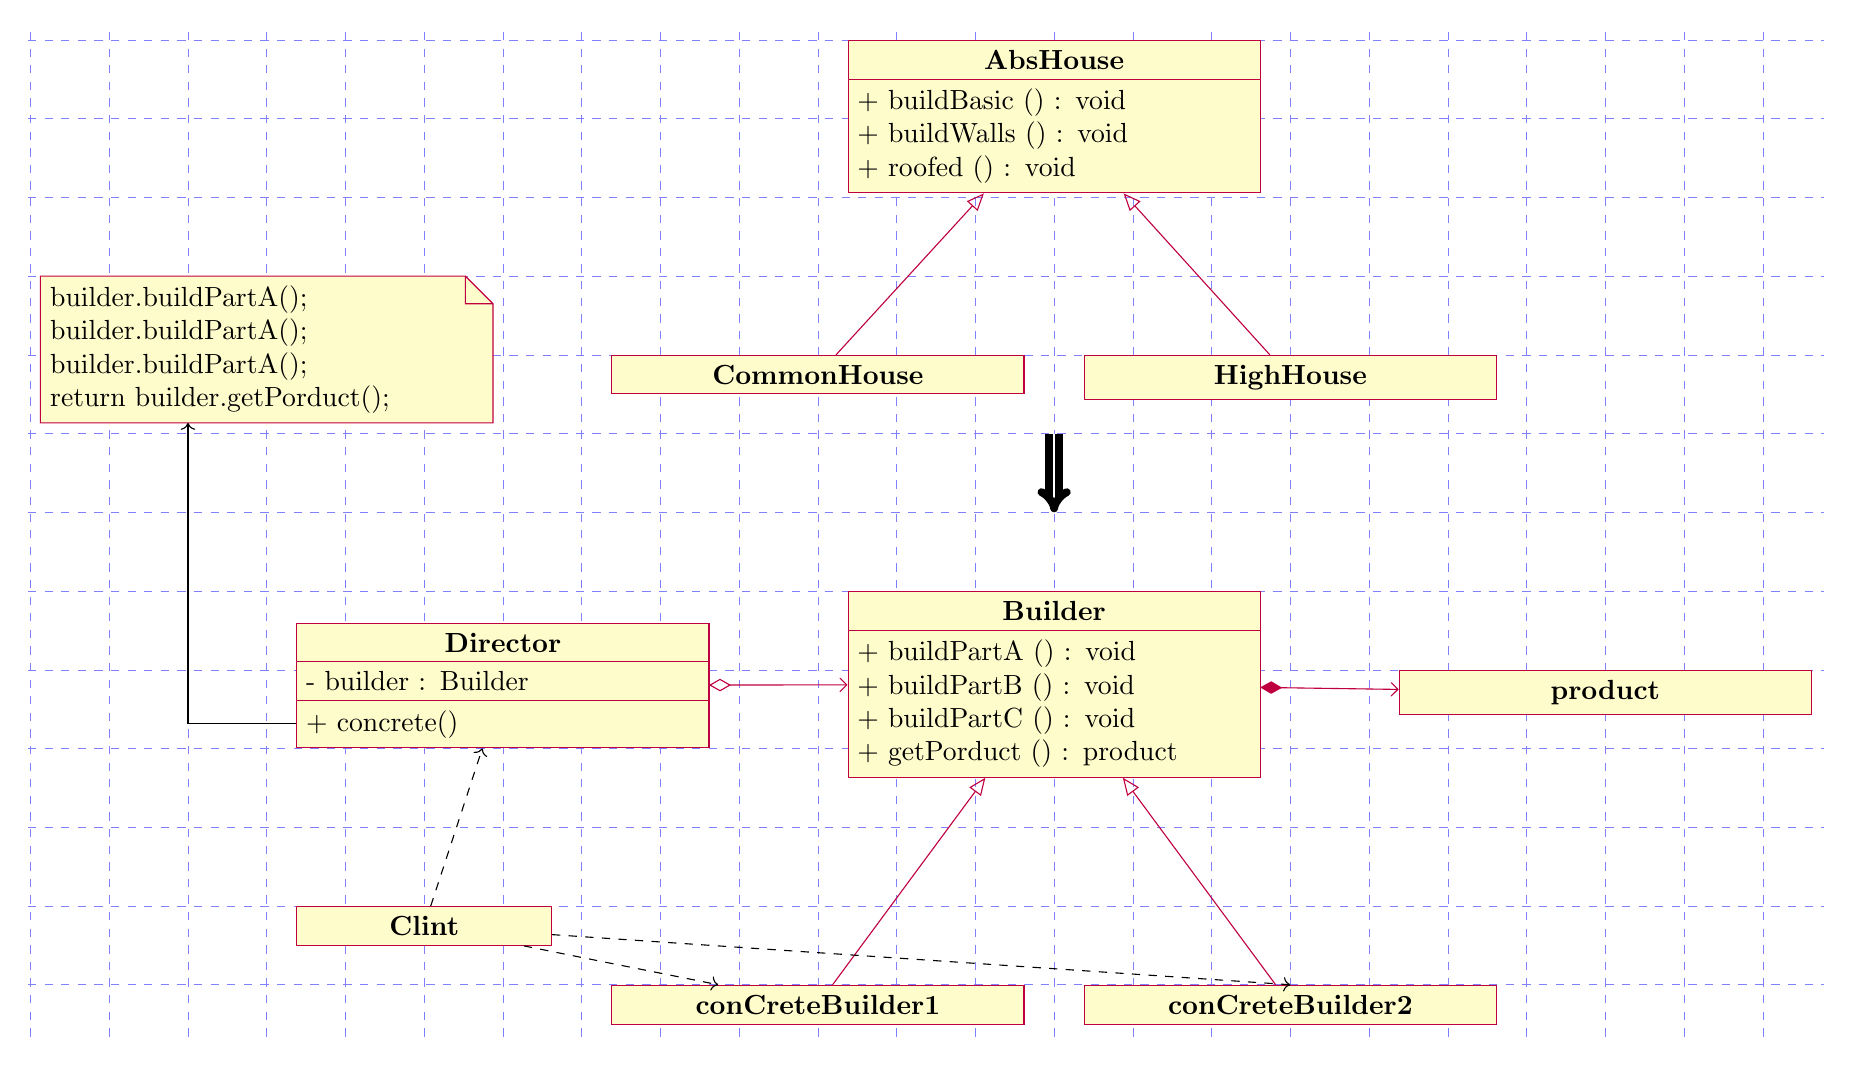
\begin{tikzpicture}[show background grid]
        \begin{class}[text width=5cm]{AbsHouse}{0,0}
            \operation{+ buildBasic () : void}
            \operation{+ buildWalls () : void}
            \operation{+ roofed () : void}
        \end{class}
        \begin{class}{CommonHouse}{-3, -4}
            \inherit{AbsHouse}
        \end{class}
        \begin{class}{HighHouse}{3, -4}
            \inherit{AbsHouse}
        \end{class}

        \draw[-Implies, double,line width=0.1cm] (0,-5) -- (0,-6);
    
        \begin{class}[text width=5cm]{Builder}{0,-7}
            \operation{+ buildPartA () : void}
            \operation{+ buildPartB () : void}
            \operation{+ buildPartC () : void} 
            \operation{+ getPorduct () : product}
        \end{class}
        \begin{class}{conCreteBuilder1}{-3, -12}
            \inherit{Builder}
        \end{class}
        \begin{class}{conCreteBuilder2}{3, -12}
            \inherit{Builder}
        \end{class}
        \begin{class}{product}{7, -8}    
        \end{class}
        \composition{Builder}{}{}{product}
        \begin{class}{Director}{-7, -7.4}
            \attribute{- builder : Builder}
            \operation{+ concrete()}
        \end{class}
        \aggregation{Director}{}{}{Builder}
        
        %\node(Director) [below left=2cm and 2cm]umlnote {hello};
        \umlnote[text width =5.5cm](conreteCode) at (-10,-3)
        {
            builder.buildPartA(); \\
            builder.buildPartA(); \\
            builder.buildPartA(); \\
            return builder.getPorduct();
        };
        %\fill[red] ($(0,1)!1.5cm!(4,1)$) circle (4pt);
        
        \draw ($(Director.south west)!0.4!(Director.west)$) 
            [->]-| ($(conreteCode.south)+(-1cm,0)$);
        \begin{class}[text width = 3cm]{Clint}{-8, -11}
        \end{class}
        \draw (Clint) [dashed ,->]-- (Director);
        \draw (Clint) [dashed ,->]-- (conCreteBuilder1);
        \draw (Clint) [dashed ,->]-- (conCreteBuilder2.north);
    \end{tikzpicture}

\end{document}